\documentclass{article}

\usepackage{arxiv}

\usepackage[utf8]{inputenc} % allow utf-8 input
\usepackage[T1]{fontenc}    % use 8-bit T1 fonts
\usepackage{hyperref}       % hyperlinks
\usepackage{url}            % simple URL typesetting
\usepackage{booktabs}       % professional-quality tables
\usepackage{amsfonts}       % blackboard math symbols
\usepackage{nicefrac}       % compact symbols for 1/2, etc.
\usepackage{microtype}      % microtypography
\usepackage{lipsum}		% Can be removed after putting your text content
\usepackage{amssymb,amsmath,amsthm}
\usepackage{listings}
\usepackage{graphicx}
\usepackage{subfig}
\usepackage{apacite}
\usepackage{algorithm}
\usepackage{algorithmicx}
\usepackage{algpseudocode}
\usepackage{kbordermatrix}% http://www.hss.caltech.edu/~kcb/TeX/kbordermatrix.sty
\usepackage{todonotes}

\newtheorem{theorem}{Theorem}
\DeclareMathOperator\supp{supp}

\title{Sampling from the Bayesian poster of an agent-based model given partial observations}

%\date{September 9, 1985}	% Here you can change the date presented in the paper title
%\date{} 					% Or removing it

\author{
  Daniel Tang\\
    Leeds Institute for Data Analytics, University of Leeds, UK\thanks{This project has received funding from the European Research Council (ERC) under the European Union’s Horizon 2020 research and innovation programme (grant agreement No. 757455)}\\
  \texttt{D.Tang@leeds.ac.uk}\\
  \AND
  Nick Malleson\\
  School of Geography, University of Leeds, UK\\  
  %% examples of more authors
  %% \AND
  %% Coauthor \\
  %% Affiliation \\
  %% Address \\
}


\begin{document}
\maketitle

\begin{abstract}
The discipline of data assimilation (DA), sometimes known as data fusion, addresses the problem of how to make use of noisy, imcomplete experimental observations to provide information about unobserved properties of a dynamical system. DA has developed rapidly in some areas of research, notably weather forecasting, but relatively little progress has been made in DA techniques applicable to agent based modelling. Agent Based Models (ABMs) consist of `agents' which often make discrete choices from a number of possible actions, meaning the space of model trajectories is not continuous and we cannot use techniques based on gradient ascent, such as 4D-VAR, that require the gradient of the posterior in this space. In addition, a set of observations will typically refute the vast majority of model trajectories, making it difficult to even identify trajectories that could have given rise to the observations, and so making it challenging to use algorithms that rely on perturbing the current solution such as non-gradient optimisation or most sampling algorithms.

Here we present an algorithm that generates samples of the time evolution of an agent based model, given a set of noisy, incomplete experimental observations of the system. The algorithm approximates the set of possible trajectories as a linear program and uses an extension of the simplex algorithm to provide a proposal function for Markov-Chain-Monte-Carlo sampling.

We demonstrate the algorithm by performing data assimilation in an agent-based, spatial predator-prey model.
\end{abstract}

% keywords can be removed
\keywords{Data assimilation, Bayesian inference, Agent based model, Integer linear programming, predator prey model}

\section{Introduction}

Agent-based modelling (ABM) has become a popular tool for use in modelling systems that are driven by the behaviours and interactions of discrete, heterogeneous entities, such as human and animal systems.
Although progress has been made towards the development and adaptation of techniques to conduct parameter optimisation~\cite{thiele_facilitating_2014}, such methods are not able to dynamically optimise the model \textit{state}. 
Agent-based models (ABMs) are typically optimised once, by repeatedly comparing their outputs under various parameter configurations to some real-world data, and then used to make predictions. 
However, in many circumstances, particularly when attempting to model complex systems, natural stochasticity causes the model to diverge from the real system, regardless of how well the parameters have been optimised.
Although some studies have attempted to re-calibrate model parameters during runtime~\cite{oloo_predicting_2018, oloo_adaptive_2017}, this does not prevent the model \textit{state} from diverging.
The field of ABM has yet to develop methods that allow the model state to be updated dynamically in response to new data, which is a serious methodological drawback. 

This paper presents a new method that will allow for \textit{data assimilation} (DA) to be applied to ABMs in order to optimise the model state in response to new data that arise during runtime. The discipline of DA, sometimes known as data fusion, addresses the problem of how to make use of noisy, imcomplete experimental observations to provide information about the time evolution of unobserved properties of a dynamical system.
It is a technique that has developed rapidly in applications such as weather forecasting~\cite{kalnay_atmospheric_2003} and the earth sciences more broadly~\cite{reichle_data_2008}, but little progress has been made in developing techniques that are applicable when the dynamical system is an agent based model. DA methods typically rely on the differentiability of the model~\cite{lewis_dynamic_2006}. As ABMs consist of `agents' that often make discrete choices from a number of possible actions, the the space of model trajectories is not continuous so techniques based on gradient ascent, such as 4D-VAR, that require the gradient of the posterior in this space, cannot be used. 
In addition, a vast number of possible model trajectories will be refuted by the observations, making it challenging to use algorithms that rely on perturbing the current solution such as non-gradient optimisation or most sampling algorithms. For this reason, examples of data assimilation using well-known DA methods such as Particle Filters and variants of the Kalman Filter -- in applications such as crime~\cite{lloyd_exploring_2016}, bus routes~\cite{kieu_dealing_2020}, pedestrian dynamics~\cite{wang_data_2015, ward_dynamic_2016, clay_realtime_2020, malleson_simulating_2020} and population movement~\cite{lueck_who_2019} -- are necessarily limited to extremely small systems, quickly becoming intractable.\todo{Reviewers may want a more comprehensive lit review}

Here we present an algorithm that generates samples of the time evolution of an agent based model, given a set of noisy, incomplete experimental observations of the system. This allows for DA on an ABM by creating a posterior distribution within a reasonable amount of time. The algorithm approximates the set of possible trajectories as a linear program and uses an extension of the simplex algorithm to provide a proposal function for Markov-Chain-Monte-Carlo sampling. We demonstrate the algorithm by performing data assimilation in an agent-based, spatial predator-prey model.

\todo[inline]{NM: ``This paper has been structured as follows ... ''}

Other work on sampling from discrete sets: Discrete hit-and-run (Baumert et.al. 2009) won't work because of the extreme sparsity of feasible points. Universal hashing (Meel et.al. 2016) doesn't seem to scale to the number of dimensions (100,000s) for this application. 

\section{Formulation of the problem}
%##########################################

Broadly, this paper presents a new method that can be used to conduct data assimilation for agent-based models. The method provides a means of sampling possible ABM trajectories, confronting them with observations from the target system, and generating a posterior. This posterior provides the best estimate of the true system state. 

\subsection{Agents, States and Actions}

Formally, we define the problem as follows.
Suppose we have a timestepping ABM where agents have a finite number of possible internal states and a finite number of ways of acting on their world. Given this, we can define an ABM as:
\begin{itemize}
	\item An ordered list of agent actions $\mathcal{A} =\left< A_0 ... A_n \right>$
	
	\item An ordered list of agent states $\mathcal{S} = \left<S_0 ... S_m\right>$
	
	\item An \textit{agent timestep}, $\pi : \mathbb{Z}\times\mathbb{Z}^{m+1}\times\mathbb{Z} \to \mathbb{R}$, which defines the probability that an agent will act in a particular way such that $\pi(\psi,\Phi,a) $gives the probability that an agent in state $S_\psi$, surrounded by agents, $\Phi$, will perform action $A_a$ (where $\Phi$ is a vector whose $i^{th}$ element is the number of agents in state $S_i$ at the start of the timestep).
	
	\item An \textit{action function}, $F: \mathbb{Z} \times \mathbb{Z} \to \mathbb{Z}^{m+1}$, which defines the effect of an action on the world such that $F(\psi, a)$ returns a vector, $\Phi$, whose $i^{th}$ element gives the number of agents in state $S_i$ that result from an agent in state $S_\psi$ performing act $A_a$ (including the final state of the acting agent).
\end{itemize}

\todo[inline]{Mention that the more traditional way of defining ABMs (e.g. using objects and step functions) can be easily mapped to this formulation}

As a simple illustration, consider a simple ``cat and mouse'' ABM, which consists of just two gridsquares, left and right, within which roam a cat and a mouse. Using the definitions above, the model can be formulated as follows: 

\begin{description}

\item[Agent actions, $\mathcal{A}$.] In any given timestep, agents can either move or stay still, so $\mathcal{A} = \left<\textrm{move}, \textrm{stay still}\right> = \left<0, 1\right>$.

\item[Agent states, $\mathcal{S}$.] The cat and mouse can exist on either of the two squares, so $\mathcal{S} = \left<\textrm{left cat}, \textrm{right cat}, \textrm{left mouse}, \textrm{right mouse} \right> = \left<0, 1, 2, 3 \right>$. 

\item[Agent timestep, $\pi$.] As there are two possible actions ($\mathcal{A}=\left<0, 1\right>$) then there are two variants to the agent timestep. With respect to the \textit{move} action ($\mathcal{A}=0$), a cat moves with probability $0.5$, irrespective of other agents, while a mouse will move if there are one or more cats on the same gridsquare, otherwise it will stay still:
\[
\begin{aligned}
\pi(\psi, \Phi, 0) &=   % MOVE equation
\begin{cases}
0.5 & \text{if } \psi \in \left\{0,1\right\}\\  % IF I'm a cat (0 and 1 are both cat) then prob move is 0.5%
1 & \text{ if } \psi = 2, \Phi_1 > 0 \text{ or } \psi=3, \Phi_2 > 0\\ % mouse left & >0 cats in same square OR mouse right and >0 cats then move
0 & \text{ otherwise} %otherwise stay still
\end{cases}
\end{aligned}
\]
With respect to the \textit{stay still} action  ($\mathcal{A}=1$), the probability of the cat staying still remains at 0.5, where as the mouse remains still if there are no cats on the same grid square, otherwise it will move:
\[
\begin{aligned}
\pi(\psi, \Phi, 1) &= % STAY STILL equation
\begin{cases}
0.5 & \text{if } \psi \in \left\{0, 1\right\}\\  % IF I'm a cat (0 and 1 are both cat) then prob stay still is 0.5%
1 & \text{ if } \psi = 2, \Phi_1 = 0 \text{ or } \psi=3, \Phi_2 = 0\\ % definitely stay still if mouse and no cats in same square
0 & \text{ otherwise}
\end{cases}
\end{aligned}
\]

\item[Action function, $F$.] Expresses the movement of the agents. For example, $F(\psi=1, a=0)$ states that if there is an agent in state $\psi=1$ (\textit{right cat}) and it performs the action $a=0$ (\textit{move)} then the result is one cat in state $\psi=0$ (\textit{left cat}):  $\Phi=\{1,0,0,0\}$. The full range of possible inputs and outputs from the action function is:
\[
\begin{aligned}
F(0, 0) &= \{0,1,0,0\}\\
F(1, 0) &= \{1,0,0,0\}\\
F(2, 0) &= \{0,0,0,1\}\\
F(3, 0) &= \{0,0,1,0\}\\
F(0, 1) &= \{1,0,0,0\}\\
F(1, 1) &= \{0,1,0,0\}\\
F(2, 1) &= \{0,0,1,0\}\\
F(3, 1) &= \{0,0,0,1\}\\
\end{aligned}
\]

\end{description}

\subsection{Trajectories}

\begin{figure}
	\centering
	\resizebox{0.5\textwidth}{!}{
		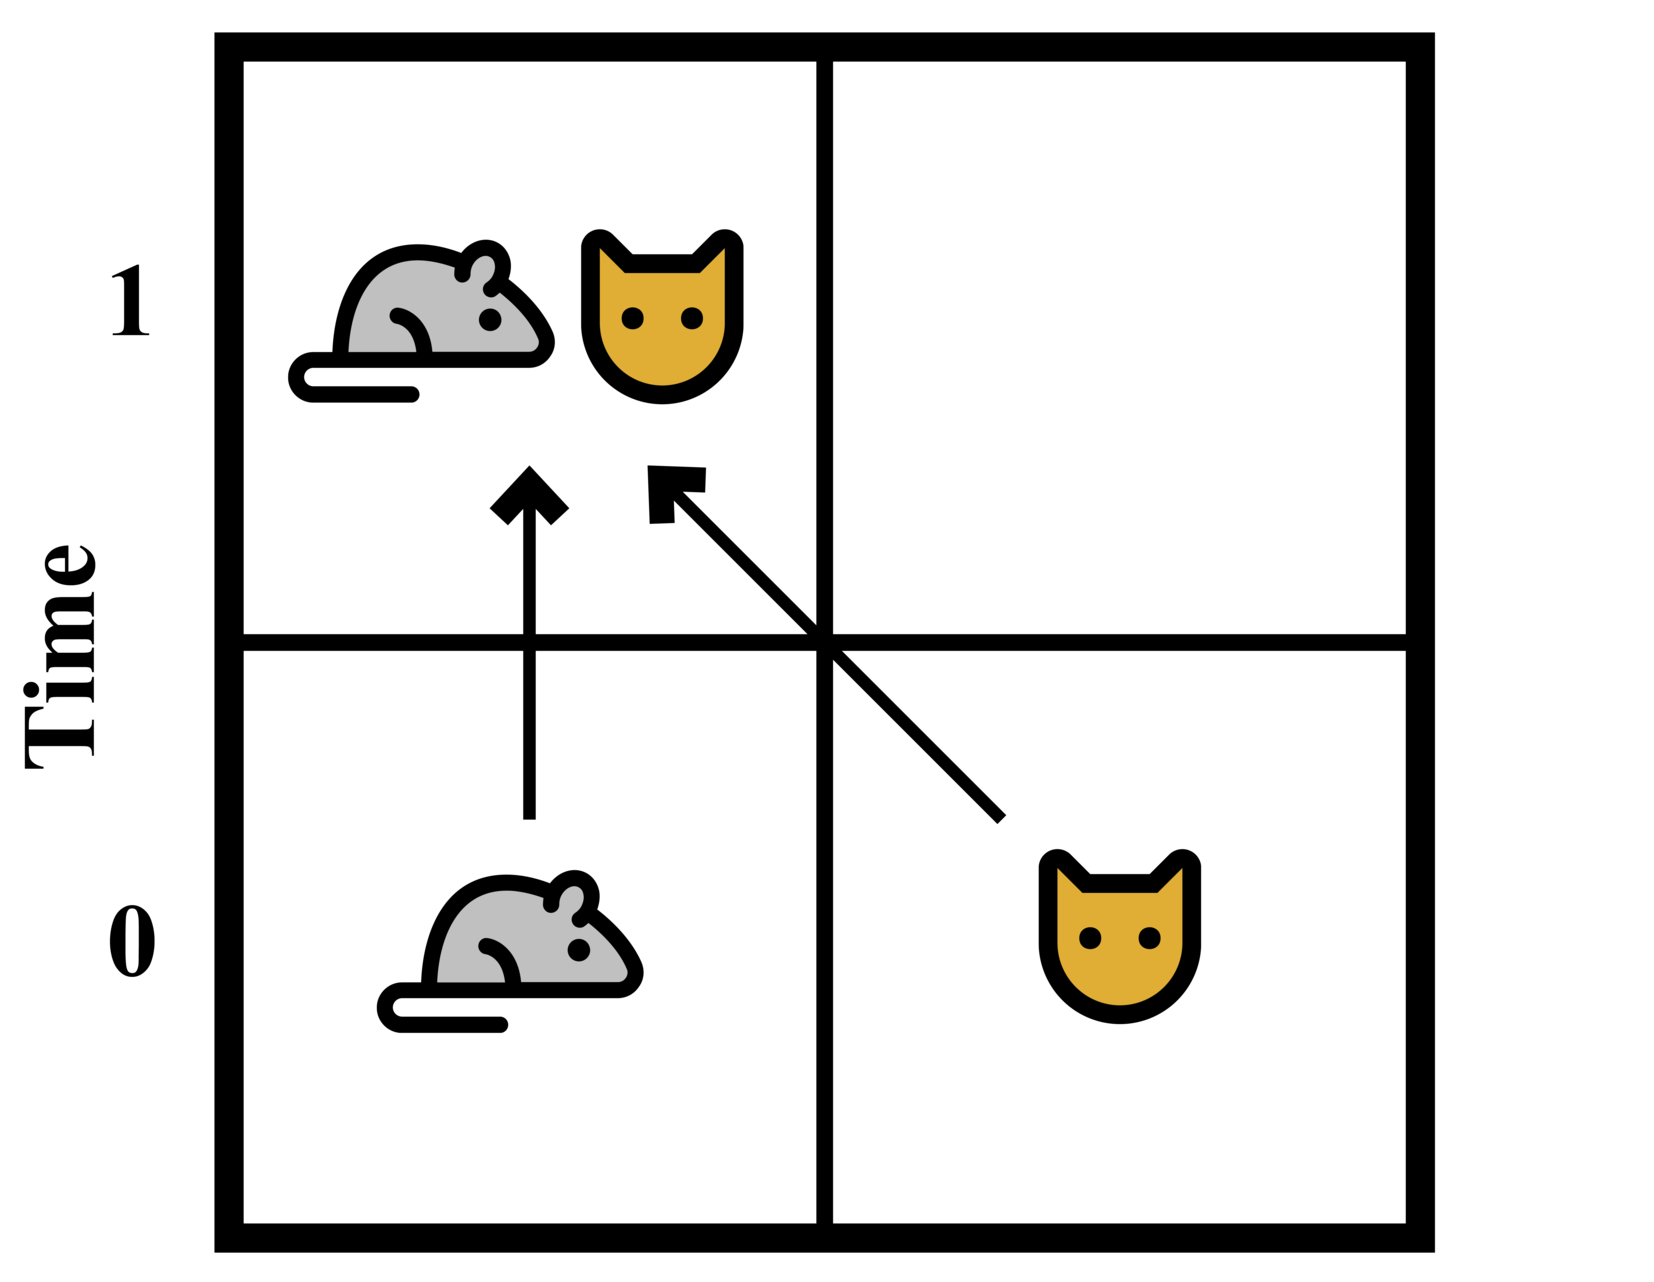
\includegraphics[scale=0.5]{figs/catMouseSm}
	}
	\caption{A simple cat and mouse model.\label{fig:AB-MCMC-1}}
\end{figure}


Let a model timestep consist of a matrix $E$ whose elements $e_{\psi a}$ are the number of agents in state $\psi$ that perform act $a$ in this timestep. For example, the timestep shown in Figure~\ref{fig:AB-MCMC-1} for the cat and mouse example would be
\[
E = \kbordermatrix{
	& A_0 & A_1 \\
	S_0 & 0 & 0 \\
	S_1 & 1 & 0 \\
	S_2 & 0  & 1 \\
	S_3 & 0 & 0 \\
}
\]
where all elements are zero except those representing agent $S_1$ (\textit{right cat}) performing action $A_0$ (\textit{move}) and agent $S_2$ (\textit{left mouse}) performing action $A_1$ (\textit{stay still}).

Finally, let a model trajectory, $T$, be an $(m\times n\times t)$ tensor consisting of $t$ model timesteps. We use the notation $T^t$ to denote the $t^{th}$ timestep matrix, $T^t_\psi$ to denote the $\psi^{th}$ row of the $t^{th}$ timestep matrix and $T^t_{\psi a}$ to denote the $a^{th}$ element of the $\psi^{th}$ row of the $t^{th}$ timestep. By convention, indices begin at 0. Note that this tensor will generally be very large for more realistic models, but also very sparse, so it can be dealt with computationally using a sparse representation.

It will occasionally be useful to refer to the set of all tensors of a given shape. For this we'll use $\mathbb{R}$ adorned with the number of elements in each index position. For example, a trajectory representing $N$ timesteps of a model with $S$ agent states and $A$ actions must be a member of the set of tensors $\mathbb{R}^N_{SA}$.

A tensor must satisfy a number of constraints in order to be a valid trajectory of an ABM. Since the elements of a trajectory are counts of agents, they must be non-negative integers. We'll call this the \textit{non-negative integer constraint} and define the set of all non-negative integer tensors
\begin{equation}
\mathcal{I}^N_{SA} = \left\{ T \in \mathbb{R^N_{SA}}: \forall t,\psi, a: T^t_{\psi a} \ge 0, T^t_{\psi a} \in \mathbb{Z}\right\}
\label{nonNegativeInt}
\end{equation}

The \textit{continuity constraint}\footnote{The continuity constraint does not mean that agents cannot leave or enter the system, only that if they do then that change must be defined as part of an action.} requires that the number of agents in each state at the end of timestep $t-1$ must be the number of agents in each state at the beginning of timestep $t$. We define the set of continuous tensors:
\begin{equation}
\mathcal{C}^N_{SA}(F) = \left\{T\in\mathbb{R}^N_{SA}:  \forall t \in 1 ... N-1:\forall \phi: \sum_{\psi, a} F(\psi, a)_\phi T^{t-1}_{\psi a} - \sum_a T^t_{\phi a} = 0\right\}
\label{continuous}
\end{equation}

So, the set of valid trajectories, $\mathcal{T}^N_{SA}(F)$, is given by the set of tensors that satisfy \eqref{nonNegativeInt} and \eqref{continuous}.
\begin{equation}
\mathcal{T}^N_{SA}(F) = \mathcal{I}^N_{SA} \cap \mathcal{C}^N_{SA}(F)
\label{SetOfTrajectories}
\end{equation}


\subsection{The posterior}

If we let $\Psi^t$ be the vector whose $\psi^{th}$ element is the number of agents in state $S_\psi$ at the beginning of timestep $t$, then the prior probability of a trajectory is
\[
P(T) =
\begin{cases}
P\left(\Psi^0 = T^0 \mathbf{1} \right) \prod_{\psi, t} P\left(T^t_{\psi} \mid \Psi^t = T^t \mathbf{1}\right) & \text{if } T \in \mathcal{T}^N_{SA}(F) \\
0 & \text{otherwise}
\end{cases}
\]
where $P(\Psi^0)$ is our prior belief about the model state at time $t=0$, and we use $\mathbf{1}$ to denote a vector whose elements are all 1.


The probability that a single agent in a given state will perform an action, given the state of the other agents, $\Psi^t$, is given by the agent timestep function, $\pi(\psi,\Psi^t,a)$, so the joint probability that $\Psi^t_\psi$ agents will perform actions $T^t_{\psi}$ in an environment of other agents $\Psi^t$, is given by the multinomial distribution
\[
P\left(T^t_{\psi} \mid \Psi^t \right) = \Psi^t_\psi!\prod_a \frac{\pi(\psi,\Psi^t,a)^{T^{t}_{\psi a}}}{T^{t}_{\psi a}!}.
\]
So the prior probability of a trajectory is
\[
P(T) =
\begin{cases}
P(\Psi^0 = T^0\mathbf{1})
\prod_{t, \psi}\left(T^t_{\psi} \cdot \mathbf{1} \right)!
\prod_a \frac{\pi(\psi, T^{t}\mathbf{1},a)^{T^{t}_{\psi a}}}{T^{t}_{\psi a}!} & \text{if } T \in \mathcal{T}^N_{SA}(F) \\
0 & \text{otherwise}\\
\end{cases}
\]

Suppose now we have a set of noisy, aggregate observations, $\Omega$, that have a likelihood function $P(\Omega|T)$. By Bayes' rule, we have
\[
P(T|\Omega) \propto P\left(\Omega \middle| T\right)P(T)
\]

Without loss of generality, we take $\Omega$ to consist of some number of observations that are independent of each other given the trajectory, so that the members $(\omega,v)\in \Omega$ consist of a stochastic observation operator $\omega$ and an observed value $v$ (which may be a vector). We write $P(\omega(T)=v)$ to denote the probability of observation operator $\omega$ making observation $v$ on trajectory $T$. So
\[
P(\Omega|T) = \prod_{(\omega,v) \in \Omega} P(\omega(T)=v)
\]

The posterior can now be written as
\begin{equation}
P(T|\Omega) \propto 
\begin{cases}
P(\Psi^0 = T^0\mathbf{1})
\prod_{(\omega,v) \in \Omega} P\left(\omega(T)=v\right)
\prod_{t, \psi, a}\left(T^t_{\psi}\cdot\mathbf{1}\right)!
\frac{\pi(\psi,T^t\mathbf{1},a)^{T^{t}_{\psi a}}}{T^t_{\psi a}!} & \text{if } T \in \mathcal{T}^N_{SA}(F) \\
0 & \text{otherwise}\\
\end{cases}
\label{posterior}
\end{equation}

In order to conduct data assimilation, we need to estimate the posterior, $P(T|\Omega)$. To do this it is necessary to sample from this distribution. This is the problem that this paper attempts to solve.
In many practical applications, sampling is difficult because the posterior has zero probability for the vast majority of tensors (i.e. most tensors are not trajectories, contain an impossible action or are refuted by the observations). Even though we can generate trajectories that fit the prior by simply performing a forward execution of the model from an initial state drawn from the prior, if the observations refute the trajectory the probability falls to zero. 
With even small numbers of observations, the probability of randomly choosing a trajectory that fits the observations becomes very small indeed. Therefore simple techniques such as rejection sampling, for example, are not practical. Techniques based on particle filtering may have more success but, for similar reasons, will likely soon reach a state containing a set of particles, none of which can be fit to the observations.

In this paper we'll show how the Metropolis-Hastings algorithm can be used to generate samples from \eqref{posterior}. The challenge will be to create a proposal function which randomly generates a proposed next sample given the current one. For example, a common strategy with Metropolis-Hastings is to generate a new sample by perturbing one or more elements of the previous sample at random. However, if we do this with an ABM trajectory it's very unlikely that the perturbed tensor will be a trajectory that contains only possible actions and satisfies the observations. So, the proposed next sample would almost certainly be rejected and we'd probably end up stuck on the first sample until we grew old.

\section{Approximating the support of the posterior}
%##########################################

We solve this problem by first approximating the support of the posterior, $\supp(P(T^t_{\psi a}|\Omega))$ (i.e. the set of trajectories that have non-zero probability).

From \eqref{posterior}
\begin{equation}
\begin{aligned}
\supp (P( T |\Omega)) = & \mathcal{T}^N_{SA} \cap \\ 
&\supp(P(\Psi^0 = T^0\mathbf{1})) \cap \\
&\bigcap_{(\omega,v) \in \Omega}  \supp\left(P\left(\omega(T)=v\right)\right) \cap \\
&\bigcap_{t, \psi, a} \left( \supp\left(\pi(\psi,T^t\mathbf{1},a)\right) \cup \left\{T:T^t_{\psi a} = 0\right\} \right)
\end{aligned}
\label{support}
\end{equation}
i.e. in order for $T$ to have non-zero posterior probability, it must be a trajectory of the ABM, it must have a start state that has non-zero prior probability, all the observation likelihoods must be non-zero and each element of $T$ must denote an agent action with non-zero probability.


\subsection{Convex $\mathbb{Z}$-polyhedra and $\mathbb{Z}$-distributions}
%################################################################
\label{BPoly}

Let a $\mathbb{Z}$-polyhedron be a set of tensors with integer elements that can be described as a set of linear constraints on the elements: 
\[
\mathcal{P^N_{SA}} = \left\{ T\in\mathbb{\mathbb{Z}}^N_{SA} : L \le \sum_{t,\psi,a} C^{\psi a}_{t} T^t_{\psi a} \le U \right\}
\]
where $L$,  $U$ and $C^{\psi a}_t$ are vectors (this is similar to the $\mathbb{Z}$-polyhedron described in \cite{quinton1996manipulating}).

From equation \ref{SetOfTrajectories} we can see immediately that $\mathcal{T}^N_{SA}$ is a  $\mathbb{Z}$-polyhedron. The supports of the prior, $P(\Psi^0)$, the observations, $P(\omega(T)=v)$, and the agent actions, $\pi(\psi,T^t\mathbf{1},a)$, can often be easily expressed as $\mathbb{Z}$-polyhedra. If this is not the case, each of the probability distributions can be expressed as computer programs. Once in this form, abstract interpretation tools\cite{cousot1977abstract} using the domain of convex polyhedra  \cite{cousot1978automatic}\cite{becchi2018efficient}\cite{fukuda2020polyhedral} can be used to construct a convex polyhedron that contains the support (note that it's fine to overestimate the support, i.e. include points that aren't in the support, but not to exclude points that are in the support. Abstract interpretation tools\cite{henry2012pagai}\cite{GN2021} are perfectly suited to this purpose). In addition, if the number of agents is very much smaller than the number of agent states (which is often the case with agent based models) then we may be willing to make the assumption that at any timestep there is at most one agent performing a given action from a given start state (i.e. $\forall \psi, a, t: T^{\psi a}_t \in \{0,1\}$). Under this assumption, which we'll call the \textit{Fermionic assumption} , the set of trajectories is a subset of the corners of the unit hypercube. Any such subset is a $\mathbb{Z}$-polyhedron.

Under the assumption that all trajectories are Fermionic, we can rewrite \eqref{support} in the form
\begin{equation}
\begin{aligned}
\supp(P( T |\Omega)) \subseteq 
& \mathcal{T}^N_{SA} \cap \\
& \mathcal{P}^N_{SA}(P(\Psi^0 = T^0\mathbf{1})) \cap\\
& \bigcap_{(\omega,v) \in \Omega}   \mathcal{P}^N_{SA}\left(P\left(\omega(T)=v\right)\right) \cap \\
& \bigcap_{t,\psi, a}
\left(\mathcal{P}^N_{SA}\left(\pi(\psi,T^t\mathbf{1},a)\right)
\cup
\left\{T: T^t_{\psi a} = 0\right\}\right)
\\
\end{aligned}
\label{polyhedralSupport}
\end{equation}

The intersection of two $\mathcal{Z}$-polyhedra is easy to construct by just concatenating the constraints
\begin{multline}
\left\{ T\in\mathbb{\mathbb{Z}}^N_{SA} : L \le \sum_{t,\psi,a} C^{\psi a}_{t} T^t_{\psi a} \le U \right\}
\cap \left\{ T\in\mathbb{\mathbb{Z}}^N_{SA} : L' \le \sum_{t,\psi,a} D^{\psi a}_{t} T^t_{\psi a} \le U' \right\} \\
= \left\{ T\in\mathbb{\mathbb{Z}}^N_{SA} : {L \choose L'}  \le \sum_{t,\psi,a} {C^{\psi a}_t\choose D^{\psi a}_t} T^t_{\psi a} \le {U\choose U'} \right\}
\end{multline}
so the only difficulty is the union in the final term of \eqref{polyhedralSupport}. To transform this into an intersection we introduce an auxiliary variable $I^t_{\psi a}$ and use the identity
\begin{multline}
\left\{ T\in\mathbb{Z}^N_{SA} : L \le \sum_{s,\phi,b} C^{\phi b}_{s} T^s_{\phi b} \le U \right\}
\cup
\left\{T: T^t_{\psi a} = 0\right\}
=\\
\left\{
T\in\mathbb{Z}^N_{SA}, I^t_{\psi a}\in\{0,1\}:\right.\\
-\infty \le \sum_{s,\phi,b} C^{\phi b}_{s} T^s_{\phi b}
+
(\overline{B}-U)I^{t}_{\psi a}
\le \overline{B},\\
\underline{B} \le \sum_{s,\phi,b} C^{\phi b}_{s} T^s_{\phi b}
+
(\underline{B}-L)I^{t}_{\psi a} \le \infty,\\
0 \le mI^t_{\psi a} - T^t_{\psi a},\\
\left. I^t_{\psi a} - T^t_{\psi a} \le 0
\right\}
\label{implication}
\end{multline}
where $m$ is the maximum value that any element of $T$ can take, the elements of $\overline{B}\in\mathbb{R}_I$ are defined as
\[
\overline{B}_i = \frac{m\sum_{s,\phi,b} \left( C^{\phi b}_{si} + \left|C^{\phi b}_{si}\right|\right)}{2}
\]
and the elements of $\underline{B}\in\mathbb{R}_I$ are defined as
\[
\underline{B}_i = \frac{m\sum_{s,\phi,b} \left(C^{\phi b}_{si} - \left|C^{\phi b}_{si}\right|\right)}{2}
\]

To see why this identity holds, note first that the constraints on $I^t_{\psi a}$ make it into an indicator variable that is 0 if $T^t_{\psi a}=0$ or 1 otherwise. When $I^t_{\psi a}=1$ the first set of constraints is equal to $\sum_{s,\phi,b} C^{\phi b}_{s} T^s_{\phi b} \le U$ and the second is equal to $L \le \sum_{s,\phi,b} C^{\phi b}_{s} T^s_{\phi b}$ so their intersection is $L \le \sum_{s,\phi,b} C^{\phi b}_{s} T^s_{\phi b} \le U$ as required, whereas when $I^t_{\psi a}=0$ we have the constraints $\underline{B} \le \sum_{s,\phi,b} C^{\phi b}_{s} T^s_{\phi b} \le \overline{B}$. But $\underline{B}$ and $\overline{B}$ are lower and upper bounds on the value of $\sum_{s,\phi,b} C^{\phi b}_{si} T^s_{\phi b}$ so this is satisfied for all trajectories, as required.

There are two things worth noting here. Firstly if we make the Fermionic assumption then $I^t_{\psi a} = T^t_{\psi a}$ and the auxiliary indicator variable becomes unnecessary. Secondly, we must impose a finite value for $m$, the maximum value that elements of the trajectory can take. In practice, this is not a problem as we can give $m$ a value such that the probability of any trajectory of interest having any element larger than $m$ is vanishingly small.

Using this transformation the support of the posterior can be reduced to a $\mathbb{Z}$-polyhedron

The idea of a $\mathbb{Z}$-polyhedron as the support for a probability distribution naturally leads to the idea of a $\mathbb{Z}$-distribution which is a discrete probability distribution defined over the members of a $\mathbb{Z}$-polyhedron. From the above, it can be seen that the posterior distribution of an ABM trajectory is a $\mathbb{Z}$-distribution.

As an illustration, consider a two-timestep trajectory of the cat and mouse model. Suppose we flip a fair coin to decide whether each agent state is occupied or empty at $t=0$ and that we observe a cat in the left grid-square at time $t=1$. Our aim is to construct a $\mathbb{Z}$-polyhedron, $\mathcal{P}^2_{4\,2}(P(T|\Omega))$, that describes the support of the posterior.

Working through \eqref{polyhedralSupport} term by term, the $\mathcal{T}^2_{4\,2}$ term is just the continuity constraints in \eqref{continuous}, which are already in linear form so we're done. The second term is the support of the prior. This constrains each agent state at $t=0$ to be at most 1, which can be expressed as
\[
\bigcap_\psi \left\{T:T^0_{\psi 0} + T^0_{\psi 1} \le 1\right\}
\]

The third term is the support of the observation. Since we observe a cat in the left grid-square at time $t=1$ we need to add the constraint
\[
T^1_{0 0} + T^1_{0 1} = 1
\]
The final term guards against impossible actions. The only impossible actions are a mouse staying put when there is a cat on the same gridsquare or moving when there are no cats, which translates to the four cases
\begin{equation}
\begin{aligned}
\supp(\pi(2,T^t\mathbf{1},0)) &= \left\{ T: -T^t_{0 0} - T^t_{0 1} \le -1 \right\}\\
\supp(\pi(3,T^t\mathbf{1},0)) &= \left\{ T: -T^t_{1 0} - T^t_{1 1} \le -1 \right\}\\
\supp(\pi(2,T^t\mathbf{1},1)) &= \left\{ T: T^t_{0 0} + T^t_{0 1} \le 0 \right\}\\
\supp(\pi(3,T^t\mathbf{1},1)) &= \left\{ T: T^t_{1 0} + T^t_{1 1} \le 0 \right\}
\end{aligned}
\label{actionConstraints}
\end{equation}
If, for simplicity, we make the Fermionic assumption by adding the constraints
\[
\forall t,\psi,a: T^t_{\psi a} \le 1
\]
then using the identity in \eqref{implication} to take the union of each constraint in \eqref{actionConstraints} with $\left\{T: T^t_{\psi a} = 0\right\}$ gives the four constraints
\[
\begin{aligned}
-T^t_{0 0} - T^t_{0 1} + T^t_{2 0} & \le 0\\
-T^t_{1 0} - T^t_{1 1} + T^t_{3 0} & \le 0\\
T^t_{0 0} + T^t_{0 1} + 2T^t_{2 1} & \le 2 \\
T^t_{1 0} + T^t_{1 1} + 2T^t_{3 1} & \le 2
\end{aligned}
\]
for each timestep $t=0$ and $t=1$.

Taken together, these constraints define a $\mathcal{B}$-polyhedron that is the set of Fermionic trajectories for the cat and mouse ABM, and when combined with \eqref{posterior} defines $P(T|\Omega)$ as a $\mathcal{B}-distribution$.

\section{Transforming between representations of a $\mathbb{Z}$-polyhedron}
%#####################################################

\todo[inline]{Brief explanation of why representing the $\mathcal{B}$-polyhedron, and transforming between representations, is needed}

Now that we can express the support of the posterior as a $\mathcal{B}$-polyhedron in the form
\begin{equation}
\supp(P(T|\Omega) \subseteq \left\{T \in \mathbb{Z}^N_{SA}: L \le \sum_{t,\psi,a} C^{\psi a}_t T^t_{\psi a} \le U \right\}
\label{bPolySupport}
\end{equation}
we describe some different ways of representing the same $\mathcal{B}$-polyhedron and methods of transforming from one representation to another. This will be useful in the development that follows.

\subsection{The standard form of a $\mathbb{Z}$-polyhedron}

Since there are many ways of representing a polyhedron, it will be useful to define a standard form when representing $\mathbb{Z}$-polyhedra. We'll use the form
\begin{equation}
\mathcal{P}(Q,N,b,L,U) = \left\{X \in \mathbb{Z}^K: X = Q{X_B\choose X_N}, X_B = b - NX_N, L \le {X_B\choose X_N} \le U, X_B\in\mathbb{Z}^I, X_N \in \mathbb{Z}^J \right\}
\label{standardpolyhedron}
\end{equation}
where $Q$ is a $K\times (I+J)$ matrix that selects $J \le K \le I+J$ elements from $(X_B|X_N)^T$ (i.e. each column of $Q$ has at most one element equal to 1, each row has exactly one element equal to 1 and all other elements are 0). We'll call the elements of $X_B$ ``basic-variables'' and the elements of $X_N$ ``non-basic variables''\footnote{The introduction of the requirement that $X_B \in \mathbb{Z}$ does not reduce expressivity as long as the elements of $N$ and $b$ can be expressed as rational numbers. In this case they can be converted to integers by multiplying each row by the product of the denominators on that row and dividing by the greatest common divisor. Once $N$ and $b$ are integer then $X_B$ is guaranteed to be integer for any $X_N\in\{0,1\}^J$.}.

Equation \eqref{bPolySupport} can easily be expressed in the form \eqref{standardpolyhedron} by ``flattening'' the trajectory, $T$, into a $J$-dimensional vector (without changing the values of the elements) using a tensor $R\in\mathbb{R}^{SA}_{NJ}$ where $J=NSA$ (i.e. for every $(t, \psi, a)$ there is exactly one $j$ such that $R^{\psi a}_{t j} = 1$ and for every $j$ there is exactly one $(t,\psi,a)$ such that $R^{\psi a}_{t j} = 1$ and all other elements are zero) so that
\[
X_N = \sum_{t,\psi,a}R^{\psi a}_t T^t_{\psi a}
\]
and letting $N$ be the $I\times J$ matrix
\[
N = \sum_{t,\psi,a} C^{\psi a}_t R^{\psi a}_t
\]
and finally letting Q be the matrix such that $X_N = Q(X_B|X_N)$ and $b = \mathbf{0}$. The constraint $X_B\in\mathbb{I}^I$ is satisfied since all the elements of $N$ are integers in our case.

\subsection{The pivot transformation}

The introduction of the matrix $Q$ in \eqref{standardpolyhedron} allows us to transform the representation without changing the $\mathbb{Z}$-polyhedron that is represented. We now describe the ``pivot transformation'' which will be a central operation in the sampling algorithm, and should look familiar to anyone acquainted with the simplex algorithm (see e.g. \cite{vanderbei2015linear}).

We begin by expressing the linear constraint in the form
\[
(I|N){X_B \choose X_N} = b
\]
where $I$ is the identity matrix.

If we let $S_{ij}$ be the permutation matrix such that
\[
{X'_B\choose X'_N} = S_{ij}{X_B\choose X_N}
\]
has the effect of swapping the $i^{th}$ element of $X_B$ with the $j^{th}$ element of $X_N$ then we have
\[
(I|N)S^{-1}_{ij}{X'_B \choose X'_N} = b
\]
(note that $S^{-1}_{ij} = S_{ij}$).

If we now pre-multiply this with the matrix 
\[
B_{ij}^{-1} =  
\begin{pmatrix}
1 &  & -\frac{N_{0j}}{N_{ij}} & & \\
  & \ddots & \vdots & &\\
 & & \frac{1}{N_{ij}} & &\\
  & & \vdots & \ddots &\\
  & & -\frac{N_{nj}}{N_{ij}} & &1\\
\end{pmatrix}
\]
it can be shown \cite{maros2002computational} that
\begin{equation}
B_{ij}^{-1}(I|N)S^{-1}_{ij} = (B_{ij}^{-1}|B_{ij}^{-1}N)S^{-1}_{ij} = (I|N')
\label{Ntransform}
\end{equation}
and so
\begin{equation}
B_{ij}^{-1}(I|N)S^{-1}_{ij}{X'_B \choose X'_N} = B_{ij}^{-1}b  = (I|N'){X'_B \choose X'_N} = b'
\end{equation}
Now, if we choose an $i$ and $j$ such that $N_{ij} = \pm 1$, then all elements of $B^{-1}_{ij}$ are integer and so all elements of $N'$ are also integer, as are the elements of $b'$. This ensures that if $X_N\in\mathbb{Z}^J$ then $X_B\in\mathbb{Z}^I$ and $X\in\mathbb{Z}^K$ as required.

So if we let
\[
Q' = QS^{-1}_{ij}
\]
we can express the original $\mathbb{Z}$-polyhedron in the equivalent form
\begin{equation}
\mathcal{P} = \left\{X\in\mathbb{Z}^K: X = Q'{X'_B\choose X'_N}, X'_B = b'-N'X'_N, S_{ij}L \le {X'_B \choose X'_N} \le S_{ij}U, X'_B \in \mathbb{Z}^I, X'_N \in \mathbb{Z}^J \right\}
\end{equation}

It is easy to see that this transformation defines an equivalence set so that, given a reference representation of a $\mathbb{Z}$-polyhedron, $\mathbb{Z}(Q,N,b,L,U)$, we can define the set of all equivalent ``pivot states'' $\mathcal{S}(Q,N,b,L,U)$.

\subsection{Removal of fixed variables}

If we use the method described in section \eqref{BPoly} to create a $\mathbb{Z}$-polyhedron of the support then each continuity constraint (and possibly some of the observation constraints) will result in elements of $X_B$ that have fixed values (i.e. $L_i = U_i$). Removing these will reduce the dimensionality of the problem and so make valid solutions easier to find.

Suppose the $i^{th}$ element of $X_B$ is fixed. If there exists some $j:N_{ij} = \pm 1$ we can perform a pivot on $(i,j)$, to swap the fixed variable with the $j^{th}$ element of $X_N$ so that the fixed variable ends up in $X_N$. The fixed variable can be removed from $X_N$ by adding the $j^{th}$ column of $N$ times the variable's fixed value to b.

\section{Sampling from a $\mathbb{Z}$-distribution}
%#################################################

Armed with the ability to express $P(T|\Omega)$ as a $\mathbb{Z}$-distribution and some tools to manipulate representations of $\mathbb{Z}$-polyhedra, we can now go about defining a Markov process which will allow us to sample from a $\mathbb{Z}$-distribution.

To do this we need to define
\begin{itemize}
\item a set of Markov states, $\mathcal{M}$

\item a probability measure $P: \mathcal{M} \to \mathbb{R}$ which gives the probability of each Markov state (this need not be normalised, though, as we'll only ever be interested in probability ratios)

\item a stochastic proposal function $f:\mathcal{M} \to \mathcal{M}$ from which we can generate transitions to a new Markov state given the current Markov state

\item a mapping $E:\mathcal{M} \to \mathbb{R}^T_{SA}$ which maps Markov states to trajectories so we can recover the sample.
\end{itemize}

In order to be useable in the Metropolis-Hastings algorithm, the proposal function, $f$, must have the following properties:
\begin{itemize}
	\item For any two Markov states there should exist a set of transitions with non-zero probability which forms a path between those states.
	
	\item For any transition from state $S_a \to S_b$ with non-zero probability, the probability of the reverse transition from $S_b \to S_a$ should also be non-zero. This allows us to attain detailed balance in the Metropolis Hastings algorithm. The average ratio of forward and backward probabilities times the ratio of start and end state probabilities should be close to 1 to ensure that a reasonable proportion of proposals are accepted.
	
	\item Given a current Markov state, there should be computationally efficient ways of generating a proposal and calculating the ratio the probability of that transition and the reverse transition. 
\end{itemize}


\subsection{The Markov states}
%#############################################

Given a $\mathbb{Z}$-polyhedron, we define a Markov state to be a pair $(X,S)$ where $X$ is a member of the $\mathbb{Z}$-polyhedron and $S$ is a pivot state that defines a standard form representation of that polyhedron.

\subsection{The probability of a Markov state}

Notice that for a given feasible solution, $X$, there are many Markov states, one for each possible pivot state. However, since the number of pivot states is the same for all feasible states we can assign to each feasible Markov state a probability $\frac{P(X)}{N}$, where $P(X)$ is the probability of solution $X$ and $N$ is the number of valid pivot states. So, the probability of being in a Markov state associated with solution $X$ (summed over all pivot states) is $P(X)$. In the Metropolis-Hastings algorithm we only ever need to calculate probability ratios so, since $N$ is independent of $X$, we never need to calculate the value of $N$\footnote{which is handy because it would be very difficult to calculate}.

\subsection{The transitions between Markov states}

\subsubsection{Bounds swaps}
Given the $X_N$ of a Markov state, a simple transition between Markov states is to swap the $i^{th}$ element of $X_N$ to it's other value while keeping the representation fixed. We'll call this a bound swap. If we're lucky the bound swap will not push $X_B$ outside its bounds and we'll have found another feasible Markov state. However, not all bound swaps are feasible in this way, and worse, there is no guarantee that given two feasible Markov states with the same representation there exists a sequence of feasible bound swaps that forms a path from one to the other.

\subsubsection{Pivot transitions}
Another simple transition between Markov states is to apply the pivot transition $S_{ij}$ to the representation for some valid $i$ and $j$. Since the variable that moves from $X_B$ to $X_N$ must end up having a value of either 0 or 1, we also specify which state this variable should end up in after the pivot. So, a pivot transition is fully defined by a triplet $(i,j,b)$.

\subsubsection{Infeasibility, infeasibility objective and potential energy}

Unfortunately, if we only allow bound swaps and pivot transitions between feasible states there is no guarantee that there is a path between any two feasible states (note that we can't pivot on the non-binary basic variables or on elements of $N$ that don't have an absolute value of 1, so we can't guarantee that all vertices of the polyhedron are reachable and so can't rely on the proof that the polyhedron is connected).

In order to deal with this, we relax the bounds on the basic variables, $L \le X_B \le U$, and include Markov states where some elements of $X_B$ go outside their bounds. This ensures a path between any two feasible states (for example, by just performing bound swaps on the elements of $X_N$) without affecting the definition of bound swaps and pivot transitions.

With this modification the sampling algorithm will sometimes return infeasible samples which don't represent valid posterior ABM trajectories. However, if we just throw these away the remaining feasible samples will have the correct distribution. So, our aim will be to ensure that the infeasible/feasible sample ratio is small enough not to excessively slow down the sampling process while being large enough to ensure proper mixing in the Markov process.

\subsection{Choosing a transition}

Now that we've defined the Markov states and the transitions between them, we next provide an algorithm to choose a proposal transition given the current Markov state. The algorithm should be able to draw a proposal from the transition-distribution and work out the ratio of probabilities of choosing a transition and its reverse transition.

The challenge here is to ensure that, during the sampling process, feasible states sometimes transition to infeasible states (in order to ensure good mixing) while ensuring that, once in an infeasible state, the sampling process quickly moves back into a (probably different) feasible state to create the next feasible sample.

In order to do this we take as our inspiration the algorithm described in \cite{maros1986general}. This algorithm is intended to be used as a ``phase I'' of the simplex algorithm (see e.g. \cite{vanderbei2015linear}) where the aim is just to find a feasible state as efficiently as possible rather than to create a Markov process. Here we present a Markov process that has a high probability of making the same transition as Maros' algorithm. Given this, we should expect the Markov process to quickly move into a feasible state.

\subsubsection{Choosing a non-basic variable: Infeasibility and potential energy}

The first step towards generating a proposal transition is to choose a non-basic variable to modify. To understand how this is done we'll first introduce a few concepts.

Given a Markov state, $\mu$, let the infeasibility of the $i^{th}$ basic variable, $\iota^\mu_i$, be defined to be equal to 0 if the variable is within its bounds or equal to the distance to the nearest bound otherwise
\[
\iota^\mu_i =
\begin{cases}
L_i-X_{Bi} & \text{if }X_{Bi}<L_i\\
X_{Bi}-U_i & \text{if }X_{Bi}>U_i\\
0 & \text{otherwise}
\end{cases}
\]
and let the total infeasibility be the sum of infeasibilities of all basic variables
\[
\iota^\mu = \sum_i \iota^\mu_i
\]
Note that the total infeasibility is piecewise linear, convex and all feasible points lie at the minimum. So, the problem is one of convex optimisation, complicated by the fact that we're only interested in integer feasible solutions. Given this,  a sensible strategy would be to somehow move down the gradient of $\iota$ towards optimal values.

The gradient of $\iota^\mu$ at any point is given by
\[
\frac{d\iota^\mu}{dX_{Bi}} = 
\begin{cases}
-1 & \text{if }X_{Bi}<L_i\\
1 & \text{if }X_{Bi}>U_i\\
0 & \text{otherwise}
\end{cases}
\]

Since $X_B = b - NX_N$, the gradient of $\iota^\mu$ with respect to $X_N$, which we'll call $D^\mu$, is given by
\[
D^\mu = \frac{d\iota^\mu}{dX_N} = \frac{d\iota^\mu}{dX_B}\frac{dX_B}{dX_N} = - \frac{d\iota^\mu}{dX_B}N
\]

Since the total infeasibility is convex, if $D^\mu_j$ is non zero we can tell which direction the $j^{th}$ non-basic variable, $X_{Nj}$, needs to be perturbed in order to potentially reduce infeasibility (or more precisely, which direction will definitely increase infeasibility). So, variables for which a bound-swap would move down the gradient $D^\mu$ are good potential candidates for perturbation compared to those that don't.

Given this, we define the potential energy of the $j^{th}$ non-basic variable to be equal to 1 if a perturbation to $X_{Nj}$ is (potentially) able to move down the gradient, and 0 otherwise.

In order to encourage the selection of columns with positive potential, the $j^{th}$ non-basic variable is chosen with probability proportional to the exponential of its potential energy times some constant $k_c$
\begin{equation}
P(j|\mu) = \frac{e^{k_cE^\mu_j}}{\sum_l e^{k_cE^\mu_l}}
\label{columnChoice}
\end{equation}

\subsubsection{Choosing a column perturbation and pivot row}

Once a non-basic variable, $X_{Nj}$, is chosen for the transition, we can choose to perform a bound-swap on $X_{Nj}$ or perform a pivot transition on the $j^{th}$ column and any row that satisfies $|N_{ij}|=1$. If a pivot is chosen, the value of the new non-basic variable needs to be chosen to be either 0 or 1. An efficient algorithm to calculate the infeasibility resulting from each of these transitions is described in \cite[Chapter~9]{maros2002computational}. For reasons that will become clear later, we also include the ``null transition'' which is a loop back to the same Markov state.

Let $\alpha^\mu_j$ be the set of destination states reachable through transitions on $X_{Nj}$. In order to encourage transitions to lower infeasibility, while maintaining the possibility of reverse transitions to allow detailed balance, a transition, $\mu\to\mu'$, is chosen with a probability proportional to the exponential of $-k_r\iota^{\mu'}$ for some constant $k_r$. i.e.
\begin{equation}
P(\mu'|j,\mu) = 
\frac{e^{-k_r\iota^{\mu'}}e^{k_cE^{\mu'}_j} }
	{\sum_{\rho \in \alpha^\mu_j}  e^{-k_r\iota^\rho}}
\label{pTransitionGivenJ}
\end{equation}

\subsubsection{Proposal function summary}

Given a transition from state $\mu$ to state $\mu' \ne \mu$ there is a unique non-basic variable $X_{Nj}$ that was involved in the transition \footnote{if $N$ is unchanged then the transition was a bound swap on the only non-basic that has changed, if $N$ changes to $N'$ then it was a pivot transition on the only $j$ that satisfies equation \eqref{Ntransform}} we'll use the notation $j^{\mu\to\mu'}$ to denote the index of this variable.

Starting from state $\mu$, the probability of proposing a transition to $\mu'$ is the probability that we choose the non-basic variable, $X_{Nj^{\mu\to\mu'}}$ then choose the state $\mu'$ from $\alpha^\mu_{j^{\mu\to\mu'}}$, so from \eqref{columnChoice} and \eqref{pTransitionGivenJ}
\[
P(\mu \rightarrow \mu') 
= 
P(\mu'|j^{\mu\to\mu'},\mu)P(j^{\mu\to\mu'}|\mu) 
=
\frac{e^{-k_r \iota^{\mu'}} e^{k_cE^{\mu'}_{j^{\mu'\to\mu}}}}
	{\sum_{\rho \in \alpha^\mu_{j^{\mu\to\mu'}}}e^{-k_r\iota^\rho}}
\frac{e^{k_c E^\mu_{j^{\mu\to\mu'}}}}
	{\sum_l e^{k_c E^\mu_l}}
\]
So, in the Metropolis-Hastings algorithm, the probability that a proposed transition, $\mu\to\mu'$, is accepted is given by
\[
\frac{P(\mu')P(\mu'\to\mu)}{P(\mu)P(\mu\to\mu')} 
=
\frac{P(\mu')}
	{P(\mu)}
\frac{e^{-k_r \iota^{\mu}}e^{k_cE^{\mu}_{j^{\mu\to\mu'}}}}
	{\sum_{\rho \in \alpha^{\mu'}_{j^{\mu'\to\mu}}}e^{-k_r\iota^\rho}}
\frac{\sum_{\rho \in \alpha^{\mu}_{j^{\mu\to\mu'}}}e^{-k_r\iota^\rho}}
	{e^{-k_r \iota^{\mu'}}e^{k_cE^{\mu'}_{j^{\mu'\to\mu}}}}
\frac{e^{k_c E^{\mu'}_{j^{\mu'\to\mu}}}}
	{\sum_l e^{k_c E^{\mu'}_l}}
\frac{\sum_l e^{k_c E^\mu_l}}
	{e^{k_c E^\mu_{j^{\mu\to\mu'}}}}
\]
However thanks to the fact that we included the null transition,  $\alpha^{\mu'}_{j^{\mu\to\mu'}} = \alpha^\mu_{j^{\mu'\to\mu}}$\footnote{since $\alpha^\mu_{j^{\mu\to\mu'}}$ describes the set of states that lie on the straight line that passes through $\mu$ and $\mu'$} the two sums over $\alpha$ cancel, leaving
\begin{equation}
\frac{P(\mu')P(\mu'\to\mu)}
	{P(\mu)P(\mu\to\mu')} 
=
\frac{P(\mu')}
	{P(\mu)}
\frac{e^{-k_r \iota^{\mu}}}
	{e^{-k_r \iota^{\mu'}}}
\frac{\sum_l e^{k_c E^\mu_l}}
	{\sum_l e^{k_c E^{\mu'}_l}}
\label{acceptance1}
\end{equation}

However, since infeasible states are thrown away in the final algorithm, we are free to assign them any probability we wish. This gives us some freedom to ensure that the algorithm spends an appropriate time in infeasible states and allows us to engineer an acceptance probability that is convenient to calculate. If we let
\begin{equation}
P(\mu) = P_e(T_\mu|\Omega)e^{-k_r \iota^{\mu}} \frac{1}{n}  \sum_l e^{k_c E^\mu_l}
\label{penalty}
\end{equation}
where $T_\mu$ is the trajectory associated with Markov state $\mu$ and $P_e(T_\mu|\Omega)$ is an ``extended posterior'', which for feasible states is just the posterior given by equation \eqref{posterior}, while for infeasible states is calculated in the same way but the requirement that the trajectory belongs to $\mathcal{T}^N_{SA}(F)$ is dropped and if any of the individual probabilities is zero it is replaced by its expectation over all trajectories (with some convenient prior over trajectories, we used a uniform distribution). Notice that for feasible states $P(\mu) = P(T_\mu|\Omega)$ so if we apply this definition to all Markov states the feasible samples will be samples from the desired posterior.

Inserting \eqref{penalty} into \eqref{acceptance2} gives the final form for the acceptance
\begin{equation}
\frac{P(\mu')P(\mu'\to\mu)}{P(\mu)P(\mu\to\mu')} 
=
\frac{P_e(T_{\mu'}|\Omega)}{P_e(T_\mu|\Omega)}
\end{equation}

Notice that states with lower infeasibility and lower potential energy have higher probability, so transitions that immediately reduce infeasibility are encouraged, but so are pivots that replace high potential energy variables with low potential variables. This has the consequence that if a high potential, non-basic variable is chosen but it can't immediately reduce infeasibility, it is more likely to be made basic where it is free to change its value in subsequent transitions. This helps the process find a basis where infeasibility-reducing transitions exist.

\subsubsection{Choosing temperature}
The exponential term $e^{\frac{-E^\mu}{T}}$ in equation \eqref{penalty} is a Boltzmann distribution so $T$ can be thought of as a ``temperature'' and the sampling process will act as a thermodynamic system in equilibrium (with the posterior $P_e(T_\mu|\Omega)$ acting as an additional potential energy).  It has been shown that thermodynamic systems of this type are able to solve large integer optimisation problems \cite{kirkpatrick1983optimization}. In our case, we don't need to change the temperature during the sampling process, but we do need to choose a value of $T$ initially. Higher temperatures will increase mixing in the Markov chain, but will also increase the proportion of time spent in infeasible states so we need to find a temperature that is high enough to ensure good mixing but low enough to ensure a reasonable proportion of samples are feasible.

[TODO: Effective procedure for choosing $T$ and rationale. Choose start and target states at random and make linear probability with target state as maximum, then tune T to minimum samples to first hitting target. Repeat.
 Proportion of infeasible samples against proportion of feasible->infeasible samples. Average infeasible chain length proportion of infeasible samples/proportion of feasible->infeasible transitions.]
 
 If we first sample uniformly from the set of all states, we can get an idea of the number of states at each energy level...or, during burn-in we reduce temperature until we hit the desired proportion of (increase temp while feasible, reduce while infeasible, gradually reducing the size of the step).
 
 The ratio of $\kappa_r$ and $\kappa_c$: If $\kappa_c$ is too low, we will tend to have long infeasible runs as high potential columns will not be pivoted-in, if it is too high, then many potential transitions into infeasibility will be rejected due to the increase in potential energy. If $\kappa_r$ is to high (absolute value) then transitions into infeasibility will not be proposed often enough, if too low then potential transitions back into feasibility may be ignored even when available. The ratio is the ratio of the energy in an infeasible variable and a high-potential column....how important is reducing infeasibility against reducing potential energy?...

\section{Results}

\section{Further work}
\subsection{Abstract interpretation using convex polyhedra}

In many cases a $\mathcal{B}$-polyhedron of the set of Fermionic trajectories in the support of the prior, observations and timestep of an agent can easily be constructed by hand in the form of a set of linear inequalities. In some cases, however, it may be less obvious how to construct this. In this case the linear inequalities can be constructed automatically from a computer program that calculates the function whose support we're trying to find.





The first two terms in equation \eqref{support} consists of the supports of computer programs whose inputs are ABM trajectories and whose outputs are given, i.e. the set of trajectories that, when passed to a computer program, would produce a given output.

Calculating the support of a computer program for a given output is, in full generality, NP-complete\footnote{Consider, for example, a program that accepts an assignment of variables to truth values, and returns true if that assignment satisfies a Boolean formula. Deciding whether the support of this program, given that it returns true, is empty or not is equivalent to solving the Boolean satisfiability problem, which is known to be NP-complete\cite{cook1971complexity}} but it is possible to use a technique known as \textit{abstract interpretation}\cite{cousot1977abstract} to efficiently calculate a superset of the support. So, given a computer program $\rho$, we can calculate a set $\mathcal{P}(\rho, v)$ such that
\[
\supp(P(\rho(.)=y)) \subset \mathcal{P}(\rho, v)
\]
Tools to perform abstract interpretation already exist (e.g. PAGAI\cite{henry2012pagai}) and are used widely in applications such as the verification of safety critical systems\cite{blanchet2003static} and in practice $\mathcal{P}(\rho, v)$ is often reasonably tight (i.e. most members of $\mathcal{P}(\rho, v)$ are in $\supp(P(\rho(.)=y))$). For our application we choose to express $\mathcal{P}(\rho, v)$ in terms of a set of linear inequalities on $\rho$'s inputs, this corresponds to the abstract domain of convex polyhedra\cite{cousot1978automatic}\cite{becchi2018efficient}. Calls to the random number generator can be dealt with in the abstract domain by generating a new variable, $r$, that satisfies $0 \le r < 1$ for each call to \texttt{Random()}. These can either be left in as ``auxiliary'' variables in the same way as slack variables, or removed as soon as the variable goes out of scope by finding the convex hull of the projection into a lower dimensional space (this can be done using the double description method\cite{motzkin1953double}).


Constraining our proposal function to members of the superset in equation \eqref{linearSupport} instead of the true support won't affect the stationary distribution of the Markov Chain. If the proposal function happens to return a trajectory that isn't in $\supp(P(\rho(.)=y))$ then it will just be rejected. This is fine as long as we generate acceptable proposals at a reasonable rate.

\section{Conclusion}

\section{Notes}


%\bibliographystyle{unsrtnat}
%\bibliographystyle{apalike} 
\bibliographystyle{apacite}
\bibliography{references}

\end{document}
